%=========================================
% 	   Cloud Native     		 =
%=========================================
\chapter{Cloud Native}

In diesem Kapitel gehen wir auf die Definition von Cloud-Native Architekturen ein, grenzen sie von anderen Absätzen ab und betrachten wichtige Eigenschaften. Abschließend beschäftigen wir uns mit den Vor-und Nachteilen und den typischen Einsatzgebieten.

\section{Cloud Computing}
Bevor wir uns mit Cloud-Native auseinandersetzten können, müssen wir uns zuerst mit dem Cloud Computing beschäftigen, da es nämlich die Basis für diese Architekturen bildet und sie maßgeblich beeinflusst. Die NIST Definition von Cloud Computing enthält die wichtigsten Merkmalen.

Cloud computing is a model for enabling ubiquitous, convenient, on-demand network access to a shared pool of configurable computing resources (e.g., networks, servers, storage, applications, and services) that can be rapidly provisioned and released with minimal management effort or service provider interaction. This cloud model is composed of five essential characteristics, three service models, and four deployment models. TODO

Entscheidend für Cloud-Native ist nun die schnelle Bereitstellung von Resourcen, denn dies eröffnet neue Möglichkeiten hinsichitlich der Skalierbarkeit und hat dadurch einen starken Einfluss auf die Architekturen.

\section{Definition Cloud Native}
Was genau Cloud-Native ist und wie man es definieren kann ist schwierig, da der Begriff noch relativ neu ist. Eine erste Version einer Definition kommt von der Cloud Native Computing Foundation, einer Organisation, die als Vorreiter in Sachen Cloud-Native gilt.

CNCF Cloud Native Definition v1.0

Cloud native Technologien ermöglichen es Unternehmen, skalierbare Anwendungen in modernen, dynamischen Umgebungen zu implementieren und zu betreiben. Dies können öffentliche, private und Hybrid-Clouds sein. Best Practices, wie Container, Service-Meshs, Microservices, immutable Infrastruktur und deklarative APIs, unterstützen diesen Ansatz.

Die zugrundeliegenden Techniken ermöglichen die Umsetzung von entkoppelten Systemen, die belastbar, handhabbar und beobachtbar sind. Kombiniert mit einer robusten Automatisierung können Softwareentwickler mit geringem Aufwand flexibel und schnell auf Änderungen reagieren.

Die Cloud Native Computing Foundation fördert die Akzeptanz dieser Paradigmen durch die Ausgestaltung eines Open Source Ökosystems aus herstellerneutralen Projekten. Wir demokratisieren modernste und innovative Softwareentwicklungs-Patterns, um diese Innovationen für alle zugänglich zu machen.

TODO wichtigsten punkte nennen


\section{Microservices}
TODO definition
warum braucht man das im cloud native bereich
Eigenschaften, Vorteile
- um diese microservices zu verwalten werden ... TODO\\
\\
Microservices sind in Cloud Native Systemen zum Erstellen von Anwendungen ein beliebter Architekturstil. Bei dieser Architektur besteht die Software aus kleinen, unabhängigen Services bzw. Modulen, die über definierte APIs (application programming interface) kommunizieren. Jeder Service kann unabhängig von anderen Services entwickelt und bereitgestellt werden, ohne die Funktionalität anderer Services zu beeinträchtigen. Den Aufbau der Microservice-Architektur sowie die Darstellung der einzelnen unabhängigen Services sind in Abbildung \ref{micro} zu sehen.\\
\begin{figure}[bth] 
	\centering
	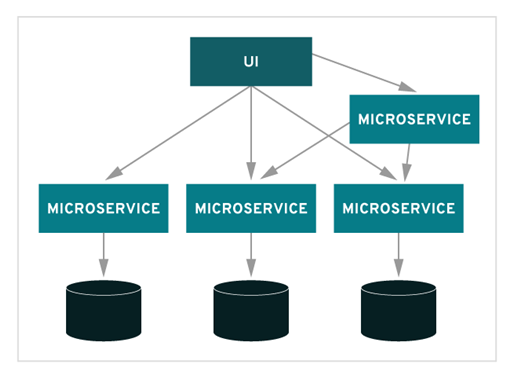
\includegraphics[width=0.6\textwidth]{Graphics/Microservice.png}
	\caption{Aufbau einer Microservice-Architektur}
	\label{micro}
\end{figure}\\
Durch die Eigenständigkeit besitzt jeder Komponentenservice seinen eigenen Code sowie seine eigene Implementierung. Jede einzelne Komponente ist auf eine Reihe von Funktionen spezialisiert, sodass sie sich auf die Lösung eines bestimmten Problems fokussiert. Wenn ein einzelner Service (z.B. hinsichtlich des Codes) zu komplex wird, kann er in kleinere Services unterteilt werden.\\
In Cloud Native Systemen sowie in der Microservice-Architektur ist die Skalierung ein wichtiger Bestandteil. Durch die Existenz der einzelnen Services können diese je nach Nachfrage unabhängig voneinander skaliert werden. Dadurch können Subsysteme, die mehr Ressourcen benötigen aufskaliert werden, ohne die gesamte Anwendung aufzuskalieren.\\
Eine weitere Eigenschaft ist die Flexibilität. Durch die Unabhängigkeit der einzelnen Services wird auch deren Verwaltung vereinfacht. Bei einer Erweiterung sowie Fehlerbehebung der Anwendung muss nur der entsprechende Service verändert werden. Dies führt dazu, dass nicht die gesamte Anwendung erneut bereitgestellt werden muss.\\
Durch die einfache Bereitstellung können z.B. neue Konzepte ausprobiert und auch schnell wieder rückgängig gemacht werden. Auf Grund der möglichen Experimente entstehen niedrige Ausfallkosten, die Aktualisierung des Codes wird erleichtert und vereinfacht das Hinzufügen neuer Funktionen.
\\

\section{Container}
TODO definition
warum braucht man das im cloud native bereich
Eigenschaften, Vorteile
Docker, Kubernetes TODO\\
\\
Auch Container sind ein wesentlicher Bestandteil von Cloud Native Systemen. \\
Ein Container ist eine Standard-Software-Einheit, die den Code und seine Abhängigkeiten verpackt, sodass Anwendungen von ihrer Ausführungsumgebung abstrahiert werden. Mit dieser Entkopplung können containerbasierte Anwendungen schnell, zuverlässig bereitgestellt und von einer beliebigen Umgebung, wie z.B. in einer öffentlichen Cloud, ausgeführt werden. In Abbildung \ref{container} ist der Aufbau einer containerbasierte Anwendung zu sehen.\\
\begin{figure}[bth] 
	\centering
	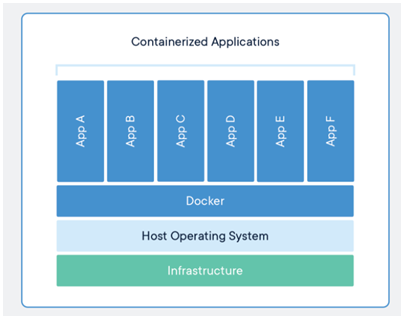
\includegraphics[width=0.6\textwidth]{Graphics/Container.png}
	\caption{Aufbau einer containerbasierte Anwendung}
	\label{container}
\end{figure}\\
Im Gegensatz zu virtuelle Maschinen wird bei der Containeriesierung weniger Speicherplatz benötigt. Hierbei handelt es sich um eine Virtualisierung auf Betriebssystemebene, da die Container direkt auf dem Kernel des Betriebssystems ausgeführt werden. Container teilen sich den Kernel des Betriebssystems, sodass sie schneller starten und im Vergleich zu einem vollständigen Betriebssystem nur einen Bruchteil an Speicher verwenden.\\
Container haben eine hohe Portabilität, sodass sie überall ausgeführt werden können. Die Softwarepakete enthalten alle Elemente, die zur Ausführung in einer beliebigen Umgebung erforderlich sind.\\
Auch bei der Containerisierung ist die Skalierbarkeit eine wichtige Eigenschaft. Denn hier besteht die Möglichkeit, dass die einzelnen Container je nach Ressourcenbedarf schnell gestartet sowie angehalten werden können. Zudem laufen sie isoliert von anderen Anwendungen.\\
\\
Es gibt verschieden Containerformate, mit deren Hilfe eine Anwendungsbereitstellung durch Containerisierung erleichtert wird. Bekannte Containerformate sind z.B. Docker und Kubernetes.\\
Docker ist ein beliebtes Open-Source-Containerformat zur Automatisierung der Bereitstellung von Anwendungen, die z.B. in der Cloud ausgeführt werden können. Docker verpackt die Software mit seinen Abhängigkeiten und alles was zur Ausführung benötigt wird in Container.\\
Wenn Anwendungen immer größer werden und die Betreibung immer komplexer wird, ist das Orchestierungssystem Kubernetes hilfreich.\\
Kubernetes ist ein Open-Source-Orchestrierungssystem zur Automatisierung z.B. zur Verwaltung, Platzierung und Skalierung von Container.

\section{Abgrenzungen}
TODO Beschreibung hinzufügen\\
gegenüber monolith\\
Definition, kurz: Eigenschaften anhand von Bild TODO\\

\subsection{Monolithische Architektur}
Bei einer monolithischen Architektur sind die Prozesse eng miteinander verbunden und werden als einziger Service ausgeführt. Wenn ein Fehler auftritt muss, im Gegensatz zu der Microservice Architektur, die gesamte Anwendung skaliert werden und nicht nur der betreffende Service. Das Hinzufügen und Verbessern von Funktionen kann je nach Aufbau der Implementierung mit zunehmender Codebasis komplexer werden sowie das Umsetzen neuer Konzepte kann je nach Aufbau der Anwendung schwieriger werden. Die Anwendungsverfügbarkeit ist im Gegensatz zu der Micorservices risikoreicher. Bei der monolithischen Architektur sind die einzelne Prozesse abhängig und eng miteinander verbunden, sodass ein einzelner Prozessausfall erhöht wird.\\
In Abbildung \ref{mono} ist der Vergleich von dem Aufbau einer monolithischen und Microservice Architektur graphisch dargestellt.
\begin{figure}[bth] 
	\centering
	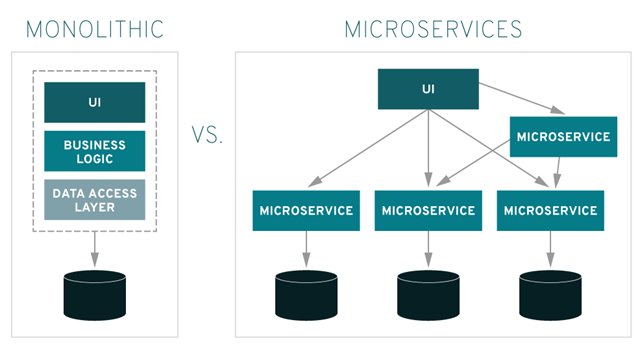
\includegraphics[width=0.9\textwidth]{Graphics/monoVsMicro.png}
	\caption{Aufbau der monolithische und der Microservice Architektur}
	\label{mono}
\end{figure}\\

\subsection{Virtuelle Maschinen}
TODO gegenüber virtualisierung\\
kurz: Definition, Vergleich/Abgrenzung anhand von Bild TODO\\
\\
Im Gegensatz zu den Container, sind virtuelle Maschinen eine Virtualisierung der gesamten Hardware bzw. Abstraktion der physischen Hardware, die einen Server in viele Server wandelt. In Abbildung \ref{vm} ist der Aufbau einer containerbasierten Anwendung im Vergleich zu einer virtuellen Maschine dargestellt.
\begin{figure}[bth] 
	\centering
	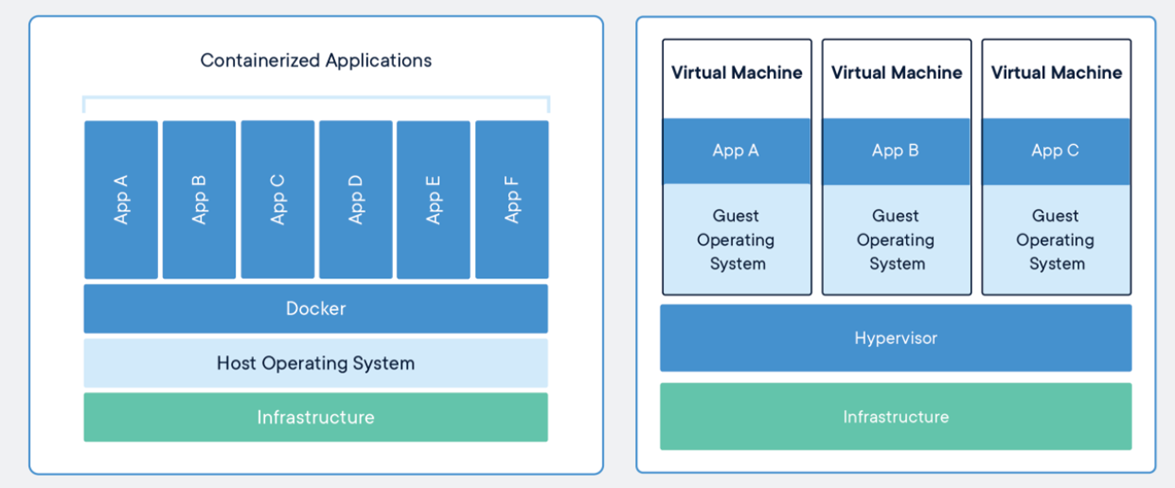
\includegraphics[width=0.9\textwidth]{Graphics/containerVsVm.png}
	\caption{}
	\label{vm}
\end{figure}\\
TODO...Vergleich genauer Beschreiben...TODO\\
- jede Vm enthält eine vollständige Kopie eines Betriebssystems, der Anwendung, notwendiger Binärdateien und Bibliotheken, eigene CPU- und Speicherressourcen -> viel Speicher\\
- Container besitzt seine Binärdateien und Bibliotheken\\

\section{Eigenschaften}
Als nächstes betrachten wir einige typischen Eigenschaften von Cloud-Native Architekturen. Im nächsten Abschnitt gehen wir dann darauf ein aus welchen Design Prinzipien hervorgehen.

1.) Globale Ebene
Cloud-Native Architekturen sind oft für eine globale Ebene ausgelegt. Das impliziert z.B. das Daten und Dienste mehrfach deployed und Daten von verschiedenen Quellen synchronisiert werden müssen.

2.) Skalierbarkeit
Die entstehenden Architekturen sind skalierbar und können eine sehr große Menge von Benutzern unterstützen. Dies ist besonders in Kombination mit der globalen Ebene, wenn man Sychronisation und Konsistenz betrachtet, eine große Herausforderung.

3.) "Built on the assumption that infrastructure is fluid and failure is constant"
Die Annahme "infrastructure is fluid" bedeutet, dass die unterliegenden Strukturen (Hardware) der nicht konstant sind. So können z.B. Recheneinheiten (CPUs) hinzukommen oder wegfallen. Diese Annahme resultiert aus der Verwendung von Cloud Technologien und bildet die Basis für das Entwerfen von skalierbaren Architekturen.
Die zweite Annahme, dass Fehler konstant auftreten, ergibt sich ebenfalls aus der Verwendung von Cloud Technologien, denn wenn eine große Anzahl von Hardwarekomponenten verwendet wird steigt die Wahrscheinlichkeit von einem Ausfall. Die Architektur muss also die Möglichkeit von Hardwarefehlern miteinbeziehen. Anders kann man dies auch Wiederstandsfähigkeit bezeichnen.

4.) Updates und Tests verlaufen unscheinbar
Die Architekturen sind so entworfen, dass Systeme, ohne Verlust von Verfügbarkeit, geupdatet und getestet werden können.

5.) Sicherheit
Sicherheit spielt eine wichtige Rolle in Cloud-Native Architekturen. Die meisten Systeme bestehen  aus vielen kleinen Teilen, für welche Zugriff auf andere Teile und Autorisierung/Authentifizierung von Benutzern geregelt werden muss.

\section{Vor- und Nachteile}
In diesem Abschnitt nennen und erklären wir einige Vor- und Nachteile von Cloud-Native Architekturen. Wir beginnen mit den Vorteilen.

1. Skalierbarkeit/Elastizität
Aus der Kombination von lose gekoppelten Komponenten und Cloud-Infrastruktur entstehen effektiv skalierbare Architekturen, denn die Komponenten können individuell hoch und runterskaliert werden. Vorraussetzung ist, dass die einzelnen Komponenten unabhängig voneinander und zustandslos sind.

2. Zuverlässigkeit/Wiederstandsfähigkeit
Cloud-Native Architekturen sind robust gegen Ausfälle der unterliegenden Strukturen. Komponenten werden überwacht und bei Bedarf neu gestartet.

3. Änderbarkeit/Wartbarkeit
Da Komponenten weitesgehend voneinander unabhängig sind, können leichter Änderungen gemacht werden, ohne andere Komponenten auch ändern zu müssen.

4. Übertragbarkeit
Durch die Verwendung von Containern und CI/CD Pipelines ist es möglich die Systeme in andere Umgebungen einfach zu installieren. Container ermöglichen dabei eine Uniforme Umgebung für die Komponenten.

prozess der pipeline, container als hauptmerkmal

5. Cloud-Native Computing Foundation
Die CNCF ist eine Organisation, die die Entwicklung im Cloud-Native Bereich unterstützt. Sie ist ein zentraler Punkt für Informationen zu Best Practices, Standards, Open-Source Projekte und Neuigkeiten im Bereich Cloud Native.

Die Liste der Nachteile ist zwar kurz, jedoch sind die Punkte hoch zu gewichten.

1. Komplexität
Wie in der Vorlesung gelernt gilt für das Entwerfen von Software-Architekturen "There is no silver bullet". Dies trifft wahrscheinlich am meisten auf Cloud Native Architekturen zu. Zwar existieren Tools und Herasngehensweisen, die in fast allen Cloud Native Architekturen zum Einsatz kommen, jedoch ist die schiere Auswahl an Möglichkeiten, die getroffen werden müssen, bereits eine Herausforderung. 
Jede Cloud Native Applikation ist ein verteiltes System, welche an sich schon sehr komplex werden können. Addiert man hierzu noch Container/Container-Orchestrierung, Sicherheitsaspekte, Datenhaltung und Skalierung/Lastenverteilung kann sehr schnell der Überblick verloren gehen. Des Weiteren ist eine solche Architektur nicht einfach zu testen, installieren oder upzudaten und es müssen weiter Tools verwendet werden, die die DevOps unterstützen.
Abschließend ist zu sagen, dass die hohe Komplexität aus den hohen Anforderungen (Skalierbarkeit, Erreichbarkeit, Sicherheit, etc.), die an Cloud Native Architekturen gestellt werden, stammt. Die Komplexität ist ein Tradeoff der bei Cloud Native Architekturen eingegangen wird, da diese in einem Zielkonflikt mit anderen Anforderungen steht. d.h. je höher der Anspruch desto komplexer gestaltet sich die Architektur.


2. Neuer Ansatz/Technologie
Die Cloud Native Computing Foundation treibt den Bereich Cloud Native stark voran, dennoch ist es ein relativ neuer Ansatz. Ständig werden neue Innovationen gemacht und bestehende Tools erweitert. Dies bedeutet, dass z.B. Fachliteratur und Erfahrene Entwickler kaum vorhanden sind. Jedoch wird wegen der hohe Komplexität eine hohe Expertise benötigt, was den Cloud-Native Bereich so schwierig macht.


\section{Einsatzgebiete}
Cloud-Native Architekturen werden derzeit meistens für Systeme benutzt, die entweder mit vielen Daten und/oder mit einer großen Anzahl von Benutzern umgehen müssen. Also generell Systeme, die ein hohes Maß an Skalierbarkeit fordern. Besonders in den Bereichen Streaming und Big Data werden häufig Cloud-Native Architekturen verwendet. 
Beispiele sind der Streaming-Dienst von Netflix sowie die Cloud Platformen von Goolge (Goolge Cloud Platform) und Amazon (AWS). In den Fällen von Google und Amazon werden Platformen angeboten die es wiederum ermöglichen Cloud-Native Applikation zu entwicklen.
Anzumerken ist, dass viele Unternehmen eine Migration ihrer Dienste in die Cloud vorgenommen haben, da die Möglichkeiten für Cloud basierte Systeme erst im letzten Jahrzent wirklich zu einer Option wurde. 